% the following command is only required if the thesis is written in german
\RequirePackage[ngerman=ngerman-x-latest]{hyphsubst}

% change to english for english theses
\documentclass[ngerman,BCOR=1.5cm,twoside]{tudscrreprt}

\usepackage[T1]{fontenc}
\usepackage[utf8]{inputenc}
\usepackage[ngerman]{babel}
\usepackage{isodate}

\usepackage[
    style=numeric-comp,
    backend=biber,
    url=false,
    doi=false,
    isbn=false,
    hyperref,
]{biblatex}
\addbibresource{bibliography.bib}
\AtEveryBibitem{%
    \clearfield{note}%
}

\usepackage[hidelinks]{hyperref} % makes all links clickable but hides ugly boxes
\usepackage[capitalise,nameinlink,noabbrev]{cleveref} % automatically inserts Fig. X in the text with \cref{..}

\usepackage[colorinlistoftodos,prependcaption,textsize=tiny]{todonotes}

\usepackage{graphicx}
\graphicspath{ {./images/} }

% if you need mathy stuff
\newtheorem{lem}{Lemma}
\crefname{lem}{Lemma}{Lemmas}
\newtheorem{thm}{Theorem}
\crefname{thm}{Theorem}{Theorems}
\newtheorem{defs}{Definition}
\crefname{defs}{Def.}{Defs.}

\usepackage{blindtext}

%\usepackage{tudscrsupervisor} % if you want to copy the sources of the task description into the thesis

\usepackage{csquotes}



\usepackage{caption}
\captionsetup{font=sf,labelfont=bf,labelsep=space}
\usepackage{floatrow}
\floatsetup{font=sf}
\floatsetup[table]{style=plaintop}
\captionsetup{singlelinecheck=off,format=hang,justification=raggedright}
\DeclareCaptionSubType[alph]{figure}
\DeclareCaptionSubType[alph]{table}
\captionsetup[subfloat]{labelformat=brace,list=off}

\usepackage{booktabs}
\usepackage{array}
\usepackage{tabularx}
\usepackage{tabulary}
\usepackage{tabu}
\usepackage{longtable}

\usepackage{quoting}

\usepackage[babel]{microtype}

\usepackage{xfrac}

\usepackage{enumitem}
\setlist[itemize]{noitemsep}

\usepackage{ellipsis}
\let\ellipsispunctuation\relax

\usepackage{listings}
\usepackage{inconsolata}

\lstdefinestyle{common-style}{
  basicstyle=\scriptsize\ttfamily,  % the size of the fonts that are used for the code
  showspaces=false,                   % show spaces adding particular underscores
  showstringspaces=false,             % underline spaces within strings
  showtabs=false,                     % show tabs within strings adding particular underscores
%  frame=tlrb,                         % adds a frame around the code
  framexleftmargin=1em,               % space between left part of frame and listing
  tabsize=2,                          % sets default tabsize to 2 spaces
  breaklines=true,                    % sets automatic line breaking
  breakatwhitespace=true,             % sets if automatic breaks should only happen at whitespace
  keywordstyle={\color{blue}\textbf}, % keywords are blue
  commentstyle={\color{gray}},        % comments
  literate={\$}{{{\$}}}1,
  basewidth=0.5em,
  breakindent=40pt,
  breakautoindent=true,
  escapechar=\&,
  aboveskip={0.1\baselineskip}
}

\lstdefinestyle{shortlisting}{
	xleftmargin=\parindent,
	frame=none,
	aboveskip=3pt,belowskip=3pt
}

\lstdefinestyle{unboxed}{
  style=common-style,
	frame=none,
}

% JastAdd
\lstdefinelanguage{AST}{
	style=common-style,
	morekeywords={abstract,rel},
	otherkeywords={::=,->,<,>},
	morecomment=[l]{//}, morecomment=[s]{/*}{*/},
}

\lstdefinelanguage{JRAG}[]{java}{
	style=common-style,
	morekeywords={abstract,public,private,boolean,aspect,null,syn,inh,coll,eq,with,int,contributes,new,return,for,if,else,this,to,true,false},
	morecomment=[l]{//}, morecomment=[s]{/*}{*/},
}

\newcommand{\lstbg}[3][0pt]{{\fboxsep#1\colorbox{#2}{\strut #3}}}
\lstdefinelanguage{diff}[]{java}{
  style=common-style,
  morecomment=[f][\lstbg{HKS07!30}]-,
  morecomment=[f][\lstbg{HKS65!30}]+,
  morecomment=[f][\textit]{@@},
  %morecomment=[f][\textit]{---},
  %morecomment=[f][\textit]{+++},
}

\lstdefinestyle{AST} { language=AST,style=common-style } 
\lstdefinestyle{JRAG} { language=JRAG,style=common-style }
\lstdefinestyle{Java} { language=Java,style=common-style }


\begin{document}

\faculty{Fakultät Informatik}
\department{}
\institute{Institut für Software- und Multimediatechnik}
\chair{Lehrstuhl für Softwaretechnologie}
\title{%
    Entwicklung eines optimalen Verfahrens zur Eroberung des
    Geldspeichers in Entenhausen
}

%% for a bachelor thesis
%\thesis{bachelor}
%\graduation[B.Sc.]{Bachelor of Science}

% for a master thesis
\thesis{master}
\graduation[M.Sc.]{Master of Science}

% for a diploma thesis
%\thesis{diploma}
%\graduation[Dipl.Inf.]{Diplom-Informatiker}

\author{Mickey Mouse}
\emailaddress[]{mickey.mouse@tu-dresden.de}
\matriculationnumber{12345678}
\matriculationyear{2016}
\dateofbirth{1.1.1990}
\placeofbirth{Dresden}
%\discipline{Distributed Systems Engineering}

\course{Distributed Systems Engineering}

\supervisor{%
    Dipl.-Inf. ABC XYZ%
    \and Dr. Sebastian Götz%
}
\professor{Prof. Dr. rer. nat habil. Uwe Aßmann}
\date{10.10.2018}
\maketitle
\newpage

\tableofcontents
\listoffigures
\listoftables

\chapter{Einleitung}\label{ch:introduction}
Thematische Einführung, Motivation

\paragraph{Ziel der Arbeit:} Konzept entwickeln, welches Zonenbasierte MRI mit Kraftsteuerung vereinigt.

Aufbau der Thesis vorstellen

In~\Cref{ch:conclusion} kommt die Zusammenfassung.

\chapter{Grundlagen}\label{ch:basics}

\section{Figures, Zitate, Mathe}
\begin{figure}[h]
\centering
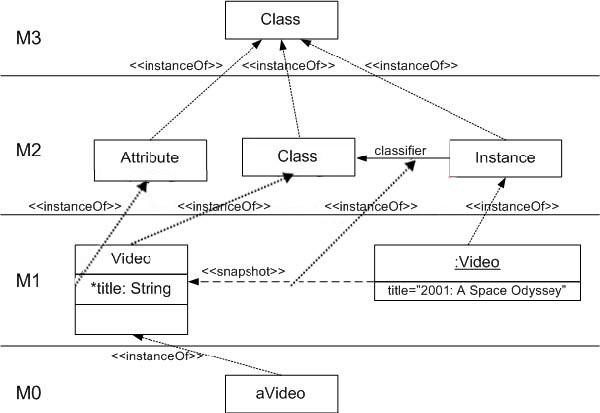
\includegraphics[scale=0.8]{OMG_MOF_4levels}
\caption{Das ist eine schlechte Grafik --- zu viele Pixel. Versuche Vektorgrafiken zu nutzen. Selbst malen geht gut mit draw.io powerpoint
  oder inkscape}\label{fig:mof}
\end{figure}

Wenn eine Abbildung verwendet wird, muss diese immer unbedingt im Text referenziert und beschrieben werden.
Z.B. so: \Cref{fig:mof}.

Zitieren geht so~\cite{haddadin2013towards}.

Math:

$A = \{x | x \in Y\}$

\begin{defs}\label{def:abc}
    A \textbf{Petrinet} is a tuple ${\Sigma = (P, T, F, W)}$.
\end{defs}

Petrinets are defined in~\Cref{def:abc}. See at the head of this document how to create your own definitions/lemma environments.


\subsection{Installation}
\textbf{Windows:} miktex

\textbf{Linux:} texlive-full

\textbf{GUI-Editor} texstudio

Konfiguration vom Editor: Preferences > Build
* default compiler: \emph{latexmk}


\section{Was ist ABC?}

\blindtext

\chapter{Problemanalyse und Modellierung}

\blindtext
\todo[inline]{Write some more}

\begin{lstlisting}[language=AST,label={lst:example-ast},caption={Example AST}]
RailwayContainer ::= Route* Region*;
abstract RailwayElement ::= <Id:int>;
Region : RailwayElement ::= TrackElement* Sensor*;
Semaphore : RailwayElement ::= <Signal:Signal>;
Route : RailwayElement ::= <Active:boolean> SwitchPosition*;
SwitchPosition : RailwayElement ::= <Position:Position>;
Sensor : RailwayElement;
abstract TrackElement:RailwayElement;
Segment : TrackElement ::= <Length:int> Semaphore*;
Switch : TrackElement ::= <CurrentPosition:Position>;
\end{lstlisting}
%
Das Listing~\ref{lst:example-ast} zeigt eine beispielhafte Grammatik, welche im Attribute im folgenden Listing genutzt wird:

\lstinputlisting[language=JRAG,style=unboxed]{code/requiredSensor.jrag}

\chapter{Erprobung der Anwendungsinstallation}\label{ch:evaluation}

\blindtext

\chapter{Zusammenfassung}\label{ch:conclusion}

\blindtext


\printbibliography[heading=bibintoc]\label{sec:bibliography}%

\appendix
\chapter{Weitere Latex-Dokumentation}
Nachdem nun der Vorspann und~-- bis auf das Literaturverzeichnis am
Ende des Dokumentes auf Seite~\pageref{sec:bibliography}~-- alle
Verzeichnisse erfolgreich ausgegeben wurden, wird nun die Verwendung
der weiteren Umgebungen und Befehle demonstriert, welche im Tutorial
\texturn{treatise.pdf} vorgestellt wurden.

\section{Referenzen und das Literaturverzeichnis}
Das Literaturverzeichnis wird auf Basis der nachfolgend verwendeten
Zitate erstellt und ist auf Seite~\pageref{sec:bibliography} zu finden.
In diesem Textabschnitt werden die zwei bekannten \LaTeX-Bücher
\cite{knuth84} und \cite{goossens94} sowie das Anwenderhandbuch
\cite{hanisch14} zitiert.p

\section{Grafiken und Tabellen in Gleitumgebungen}
Es folgt die Demonstration von Gleitumgebungen, welche sowohl für
Grafiken als auch Tabellen verwendet werden sollten. Im vorliegenden
Beispiel kann unter Umständen der Eindruck entstehen, dass diese Seite
etwas zu überladen mit Gleitobjekten ist. Dies liegt nicht an der
Verwendung der Gleitobjekte sondern vielmehr am zu geringen Textvolumen
und den eingeschränkten Möglichkeiten von \LaTeX{}, diese an geeigneten
Stellen zu platzieren.

\subsection{Abbildungen als Gleitobjekte und das Einbinden von Grafiken}
In \autoref{fig:example} wird dargestellt, wie eine Grafik im PDF"~Format
in ein Dokument eingebunden und auf diese verwiesen werden kann. Ein
Querverweis auf ein Gleitobjekt sollte im Fließtext am besten mit Befehl
\texttt{\textbackslash autoref\{\emph{<Label>}\}} erstellt werden.
Hierfür ist ein entsprechender Anker am zu referenzierenden Objekt nötig,
welcher mit dem Makro \texttt{\textbackslash label} erzeugt wird. Dabei
ist entscheidend, dass dieser Anker erst \emph{nach} der Beschriftung des
Objektes, welche mit \texttt{\textbackslash caption} zu erstellen ist,
definiert werden sollte.

\begin{figure}
\centering
\includegraphics{TUD-black}
\caption{Beispielgrafik}\label{fig:example}
\end{figure}

\subsection{Untergleitobjekte}
Nachdem nun schon eine gleitende Abbildung und zwei gleitende Tabellen
erstellt wurden, folgt jetzt noch eine gleitende Abbildung mit zwei
Unterabbildungen. Durch die drei gesetzten Anker kann im Fließtext
sowohl auf \autoref{fig:logos} als auch auf \autoref{fig:tud} sowie
\autoref{fig:ddc} verwiesen werden.

\begin{figure}
\ffigbox[\FBwidth]%
  {\begin{subfloatrow}%
    \ffigbox[\FBwidth]%
      {\fbox{\includegraphics[height=2cm]{TUD-black}}}%
      {\caption{Eine Abbildung}\label{fig:tud}}%
    \ffigbox[\FBwidth]%
      {\fbox{\includegraphics[height=2cm]{DDC-21}}}%
      {\caption{Eine weitere Abbildung}\label{fig:ddc}}%
  \end{subfloatrow}}%
  {\caption{Eine Gleitumgebung mit zwei Abbildungen}\label{fig:logos}}%
\end{figure}

\subsection{Tabellen als Gleitobjekte}
Tabellen sollten in der \texttt{table}"=Gleitumgebung gesetzt werden.
Welche Umgebung für die Tabelle selbst dabei genutzt wird ist dabei
nicht relevant. Es können sowohl die normale \texttt{tabular}"=Umgebung
als auch die Umgebungen \texttt{tabularx}, \texttt{tabulary} sowie
\texttt{tabu} für variable Spaltenbreiten bei einer fest vorgegebenen
Tabellenbreite oder jede andere Tabellenumgebung genutzt werden.
Nachfolgend wird dies an mehreren Beispielen demonstriert.

\subsubsection{Eine gleitende tabularx-Tabelle}
Es wird eine Tabelle mithilfe der \texttt{tabularx}"=Umgebung erstellt.
Zu sehen ist diese in \autoref{tab:tabularx}. Für diese werden zuvor
neue Spaltentypen definiert.

\newcolumntype{Y}{>{\hspace{0pt}}X}
\newcolumntype{D}{>{\raggedright}Y}
\newcolumntype{E}{>{\centering}Y}
\newcolumntype{F}{>{\raggedleft}Y}

\begin{table}
\begin{tabularx}{\textwidth}{@{}EEEEE@{}}
\toprule
\textbf{Problem ID} & \textbf{Basic} &
\textbf{with new probabilities} & \textbf{without duplicates in population} & \textbf{without duplicates in population + tuning} 
\tabularnewline
1 & 1.23 & 0.01 & 0 & 0
\tabularnewline
10 & 0.26 & 0.01 & 0 & 0
\tabularnewline
13 & 1.23 & 0.01 & 0 & 0
\tabularnewline
19 & 1.23 & 0.01 & 0 & 0
\tabularnewline
28 & 1.23 & 0.01 & 0 & 0
\tabularnewline
31 & 1.23 & 0.01 & 0 & 0
\tabularnewline
\bottomrule
\end{tabularx}
\caption{Eine \texttt{tabularx}"=Tabelle}\label{tab:tabularx}
\end{table}

\subsubsection{Eine gleitende tabulary-Tabelle}
Es wird eine Tabelle mithilfe der \texttt{tabulary}"=Umgebung erstellt.
Zu sehen ist diese in \autoref{tab:tabulary}.

\begin{table}
\begin{tabulary}{\textwidth}{@{}LCRJ@{}}
\toprule
\textbf{Linksbündig} & \textbf{Zentriert} &
\textbf{Rechtsbündig} & \textbf{Blocksatz} \tabularnewline\midrule
Ein linksbündiger Blindtext zur Demonstration einer L"~Spalte &
Ein zentrierter Blindtext zur Demonstration einer C"~Spalte &
Ein rechtsbündiger Blindtext zur Demonstration einer R"~Spalte &
Ein wesentlich längerer und absolut inhaltsleerer Blindtext im
Blocksatz für eine um einiges bessere Demonstration einer J"~Spalte
\tabularnewline\bottomrule
\end{tabulary}
\caption{Eine \texttt{tabulary}"=Tabelle}\label{tab:tabulary}
\end{table}

\subsubsection{Eine gleitende tabu-Tabelle}
In \autoref{tab:tabu} ist eine weitere Tabelle mit variabler Breite der
Spalten und festgelegter Gesamtbreite zu sehen, welche in der Umgebung
\texttt{tabu} gesetzt wurde. Auch für diese wird zuerst ein neuer
Spaltentyp definiert, der die Unzulänglichkeiten der Umgebung reduziert.
Mit \texttt{\textbackslash ttabbox} aus dem Paket \texttt{floatrow} wird
die Beschriftung auf die Breite der Tabelle begrenzt.

\makeatletter
\newcolumntype{Z}{}
\renewcommand*{\NC@rewrite@Z}[1][]{%
  \NC@find>{\hspace{0pt}}X[#1]<{\@finalstrut\@arstrutbox}%
}
\makeatother

\begin{table}
\ttabbox{%
  \begin{tabu} to .8\textwidth {@{}Z[3,l]Z[3,c]Z[3,r]Z[2,j]@{}}
    \toprule
    \textbf{Linksbündig} & \textbf{Zentriert} &
    \textbf{Rechtsbündig} & \textbf{Blocksatz} \tabularnewline\midrule
    Ein linksbündiger Blindtext zur Demonstration einer Z[l]"~Spalte &
    Ein zentrierter Blindtext zur Demonstration einer Z[c]"~Spalte &
    Ein rechtsbündiger Blindtext zur Demonstration einer Z[r]"~Spalte &
    Ein Blindtext im Blocksatz innerhalb einer Z"~Spalte
    \tabularnewline\bottomrule
  \end{tabu}%
}{%
  \caption[Eine \texttt{tabu}"=Tabelle]{%
    Eine \texttt{tabu}"=Tabelle in Verbindung mit dem Befehl
    \texttt{\textbackslash ttabbox}, welcher vom Paket \texttt{floatrow}
    für Beschriftungen in Objektbreite bereitgestellt wird%
  }%
  \label{tab:tabu}%
}
\end{table}

\section{Zitate}
Bei der Verwendung von wörtlichen Zitaten sollten diese als solche
gekennzeichnet werden.
\enquote{Dies ist ein zugegebenermaßen nicht sehr sinnvolles Zitat.}
\cite[58]{hanisch14}
Für eine möglichst gut nachvollziehbare Referenz sollte nicht nur
das Werk selber sondern zumindest die Seitenzahl und gegebenenfalls
der Absatz der originalen Textstelle angegeben werden.
\begin{quoting}
\enquote{%
  Dies ist ein noch sinnloseres Zitat. Allerdings wird zumindest die
  Wirkung der Umgebung \texttt{quoting} bei der Absatzauszeichnung
  deutlich.

  Wie zu sehen ist, wird der zweite Absatz~-- wie jeder weitere~--
  aufgrund der Option \texttt{parskip=false} eingezogen.
}
\cite[sinngemäß nach][\pno{} 12, zweiter Absatz]{hanisch14}
\end{quoting}
Ebenfalls sollten sinngemäße Zitate mit einer möglichst genauen Referenz
angegeben werden. Dies kann im Laufe der Arbeit auch für einen selbst von
Vorteil sein, wenn beispielsweise die originale Textpassage noch einmal
analysiert werden soll.


\confirmation

\end{document}
